\appendix{Anexo: Abordagem \textit{SMarty}}
\label{sec:Abordagem_SMarty}

%\section{Apresentação}
A abordagem \textit{SMarty} \cite{BeraICEIS2015}; \cite{GeraldiICEIS2015}; \cite{MarcolinoEtAl2014}; \cite{MarcolinoICEIS2014}; \cite{MarcolinoSEKE2013}; \cite{OliveiraJuniorJUCS2010} possibilita o gerenciamento de variabilidades em LPSs modeladas em \textit{Unified Modeling Language} (UML), a partir de um conjunto de estereótipos e diretrizes, que aplicadas aos elementos dos modelos, permitem a representação das variabilidades.

Os estereótipos fornecidos por \textit{SMarty} estão organizados em um perfil UML denominado \textit{SMartyProfile} (apresentado abaixo) e em um conjunto de diretrizes para auxiliar na identificação, delimitação e representação das variabilidades, com base em tais estereótipos, denominado \textit{SMartyProcess}.

\begin{landscape}
	\begin{figure}[]
		\centering		
		\caption{Versão 5.2 do \textit{SMartyProfile}, com suporte a Componentes, Portas, Interfaces e Operações \cite{Bera2015}.}	
		\label{SMartyProfile}
		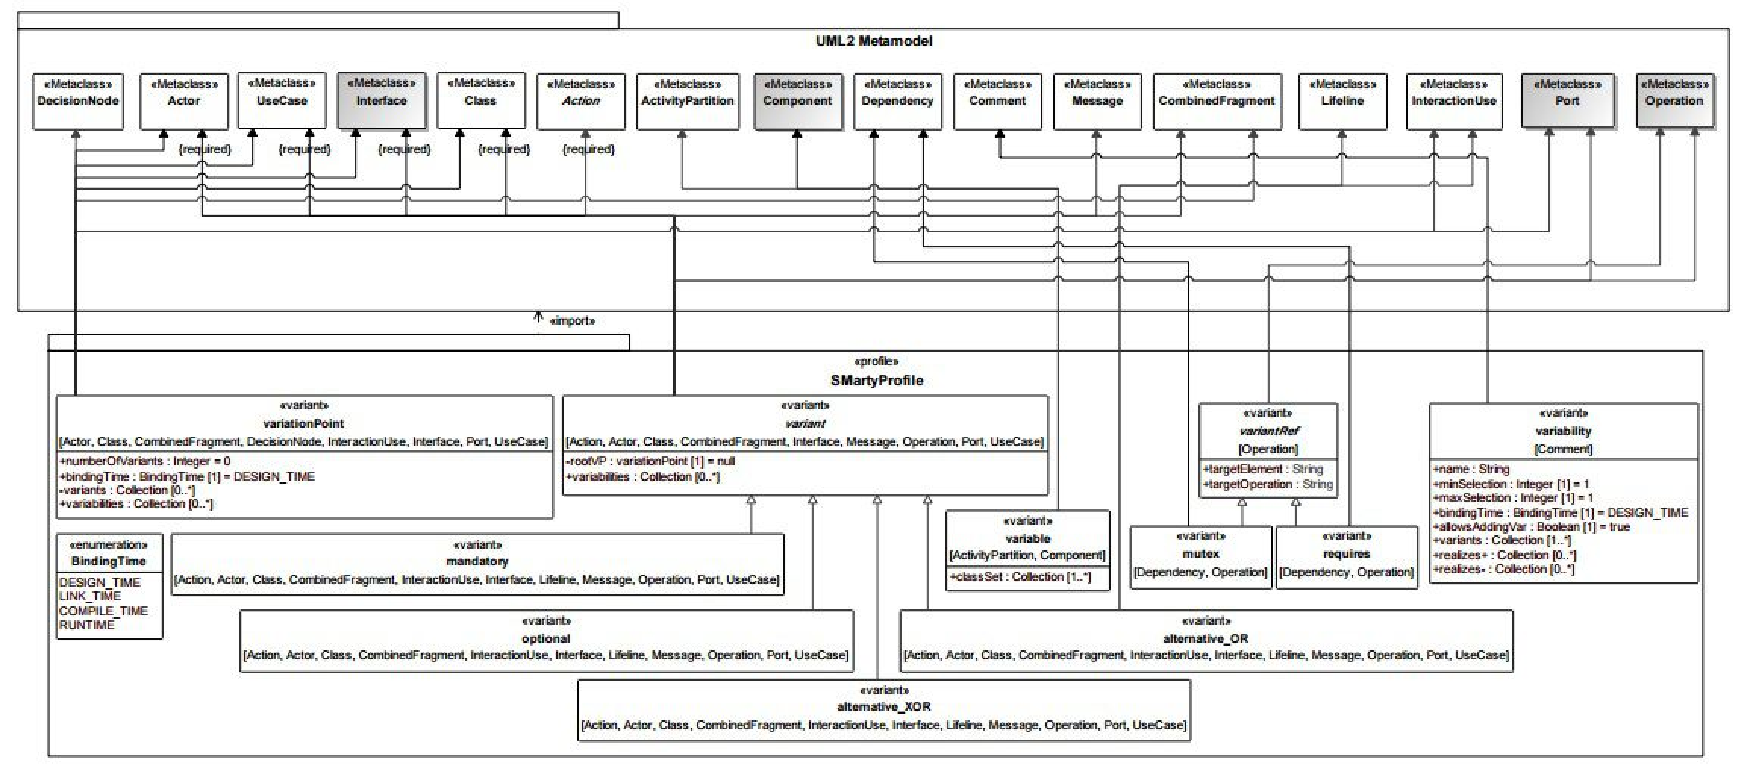
\includegraphics[height=16cm, width=22cm]{SMartyProfile5_2.pdf}
	\end{figure}	
\end{landscape}

O \textit{SMartyProfile} é uma extensão dos metamodelos da UML, versão 2.5. É possível perceber todos os estereótipos suportados pelo perfil na região inferior da \ref{SMartyProfile}. Os estereótipos representam conceitos característicos de LPS, como variabilidades, pontos de variação e variantes nos modelos UML. A seguir, são apresentados os estereótipos do \textit{SMartyProfile}:

$<<\textbf{\textit{variability}}>>$ estereótipo de variabilidade. Esse estereótipo é uma extensão da metaclasse UML \textit{Comment}, para representar explicitamente as variabilidades nos modelos UML. Tal estereótipo apresenta os seguintes meta-atributos;
\begin{itemize}
	\item \textbf{\textit{name}:} nome utilizado para referenciar uma variabilidade;
	\item \textbf{\textit{minSelection}:} corresponde ao número mínimo de variantes selecionadas para resolver um ponto de variação e/ou uma variabilidade;
	\item \textbf{\textit{maxSelection}:} corresponde ao número máximo de variantes selecionadas para resolver um ponto de variação e/ou uma variabilidade;
	\item \textbf{\textit{bindingTime}:} corresponde ao momento de resolução da variabilidade. Os possíveis momentos de resolução são representados pela classe de enumeração BindingTime;
	\item \textbf{\textit{allowsAddingVar}:} indica se novas variantes podem ser incluídas após a resolução de uma variabilidade;
	\item \textbf{\textit{variants}:} coleção de instâncias, associadas à variabilidade; e
	\item \textbf{\textit{realizes}:} coleção de variabilidades de modelos de menor nível que realiza a variabilidade.
\end{itemize}

$<<\textbf{\textit{variationPoint}}>>$ estereótipo de ponto de variação. Esse estereótipo estende as metaclasses \textit{Actor}, \textit{Class}, \textit{CombinedFragment}, \textit{DecisionNode}, \textit{InteractionUse}, \textit{Interface}, \textit{Port}, \textit{UseCase} e possui os seguintes meta-atributos:
\begin{itemize}
	\item \textbf{\textit{numberofVariants:}} número de variantes associadas ao ponto de variação;
	\item \textbf{\textit{bindingTime:}} estabelece o tempo de resolução do ponto de variação.  Os possíveis tempos de resolução são determinados pela classe de enumeração \textit{BindingTime} do \ref{SMartyProfile};
	\item \textbf{\textit{variants}:} coleção de instâncias de variantes associadas ao ponto de variação; e
	\item \textbf{\textit{variabilities}:} coleção de variabilidades associadas com este ponto de variação.
\end{itemize}

$<<\textbf{\textit{variant}}>>$ estereótipo de variante. Tal estereótipo é especializado em outros quatros estereótipos ($<<\textbf{\textit{mandatory}}>>$, $<<\textbf{\textit{optional}}>>$, $<<\textbf{\textit{alternative\_XOR}}>>$ e $<<\textbf{\textit{alternative\_OR}}>>$), estende as metaclasses \textit{Action}, \textit{Actor}, \textit{Class}, \textit{CombinedFragment}, \textit{Interface}, \textit{Message}, \textit{Operation}, \textit{Port}, \textit{UseCase} e possui os seguintes meta-atributos:
\begin{itemize}
	\item \textbf{\textit{rootVP}:} representa o ponto de variação ao qual a variante está associada; e
	\item \textbf{\textit{variabilities}:} coleção de variabilidades ao qual a variante está associada.
\end{itemize}

$<<\textbf{\textit{mandatory}}>>$ estereótipo de variante obrigatória. Isso indica que essa variante sempre deve estar na resolução de um ponto de variação e/ou variabilidade associado(a). As seguintes metaclasses são estendidas por esse estereótipo: \textit{Action}, \textit{Actor}, \textit{Class}, \textit{CombinedFragment}, \textit{InteractionUse}, \textit{Interface}, \textit{Lifeline}, \textit{Message}, \textit{Operation}, \textit{Port}, \textit{UseCase};

$<<\textbf{\textit{optional}}>>$ estereótipo opcional, na resolução de um ponto de variação e/ou variabilidade associado(a). Tal estereótipo é uma extensão das seguintes metaclasses: \textit{Action}, \textit{Actor}, \textit{Class}, \textit{CombinedFragment}, \textit{InteractionUse}, \textit{Interface}, \textit{Lifeline}, \textit{Message}, \textit{Operation}, \textit{Port} e \textit{UseCase};

$<<\textbf{\textit{alternative\_XOR}}>>$ estereótipo que indica a existência de um grupo de variantes exclusivas, do qual a variante marcada com tal estereótipo faz parte. Isso significa que apenas uma variante desse grupo pode ser selecionada para a resolução de um ponto de variação e/ou variabilidade associado(a). Esse estereótipo é uma extensão das metaclasses \textit{Action}, \textit{Actor}, \textit{Class}, \textit{CombinedFragment}, \textit{InteractionUse}, \textit{Interface}, \textit{Lifeline}, \textit{Message}, \textit{Operation}, \textit{Port} e \textit{UseCase};

$<<\textbf{\textit{alternative\_OR}}>>$ estereótipo que indica que a variante pertence a um grupo de variantes inclusivas. Isso significa que diferentes combinações de variantes inclusivas podem ser selecionadas para a resolução de um ponto de variação e/ou variabilidade associado(a). Esse estereótipo é uma extensão das metaclasses \textit{Action}, \textit{Actor}, \textit{Class}, \textit{CombinedFragment}, \textit{InteractionUse}, \textit{Interface}, \textit{Lifeline}, \textit{Message}, \textit{Operation}, \textit{Port} e \textit{UseCase};

$<<\textbf{\textit{mutex}}>>$ estereótipo que representa o relacionamento mutuamente exclusivo entre variantes. Isso significa que a escolha de uma variante desse relacionamento exige a não-escolha da outra variante do relacionamento. Tal estereótipo é uma extensão das metaclasses \textit{Dependency} e \textit{Operation};

$<<\textbf{\textit{requires}}>>$ estereótipo que representa um relacionamento de complemento entre duas variantes. Isso significa que a escolha de uma variante desse relacionamento requer a seleção da outra variante relacionada. As metaclasses \textit{Dependency} e \textit{Operation} são estendidas por $<<\textit{requires}>>$;

$<<\textbf{\textit{variable}}>>$ estereótipo extensão das metaclasses \textit{ActivityPartition} e \textit{Component}, que indica a existência de classes com variabilidades explícitas em um componente. O atributo \textit{classSet} representa a coleção de instâncias das classes variáveis existentes no componente.

Os estereótipos do \textit{SMartyProfile} permitem a representação explícita dos conceitos de LPS e possibilitam que o processamento automatizado de modelos UML, realizado por ferramentas de modelagem UML, também considere as características de LPS.

A \ref{SMartyProfileVersoes} exibe uma visão geral da abordagem SMarty.

\begin{figure}[!htb]
	\centering		
	\caption{Visão Geral SMarty 5.2 \cite{Bera2015}.}	
	\label{SMartyProfileVersoes}
	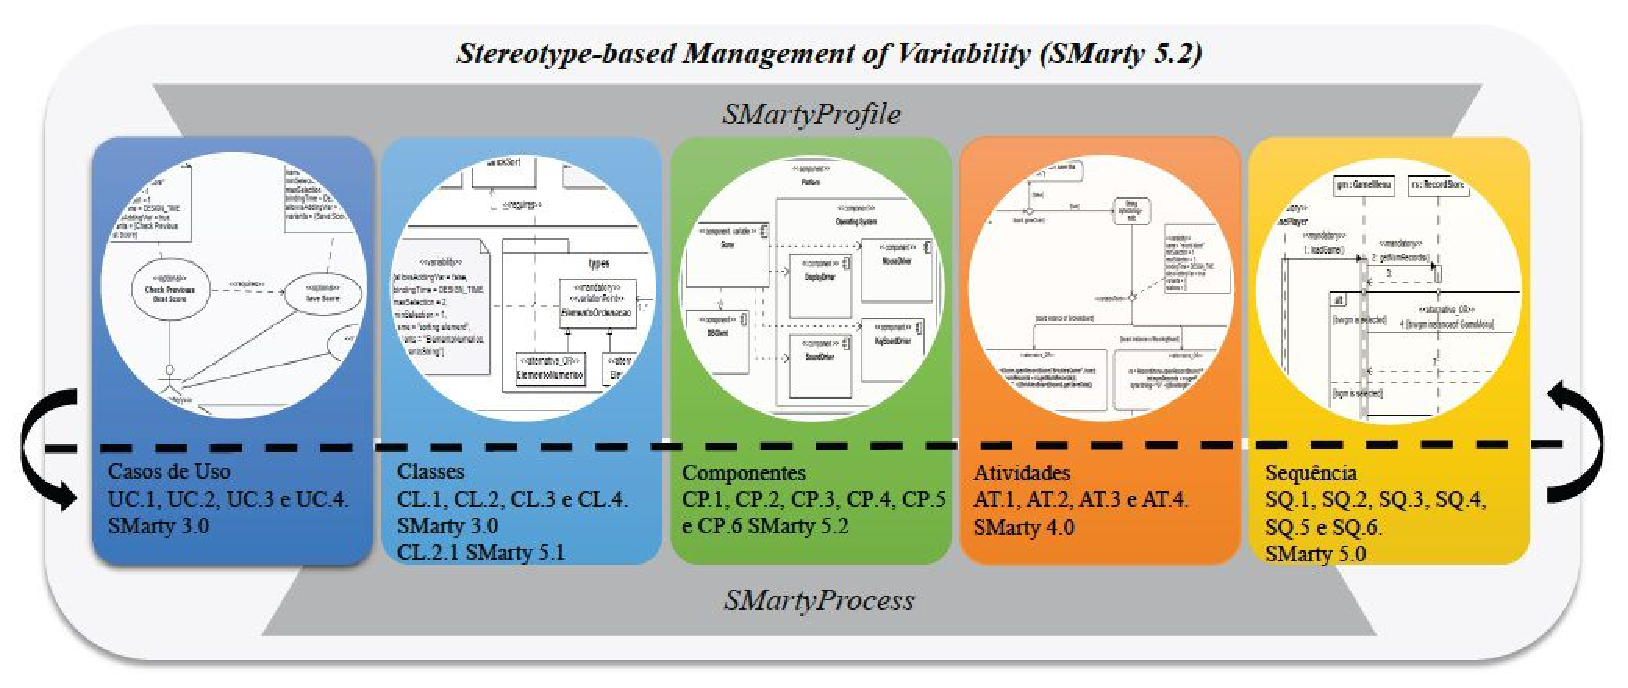
\includegraphics[height=10cm, width=16cm]{SMarty_Versao_Total_editado.pdf}
\end{figure}

A \ref{SMartyProfileVersoes} possibilita visualizar os modelos UML para o qual a abordagem \textit{SMarty} oferece suporte. Para cada modelo suportado, tem-se os estereótipos, definidos pelo \textit{SMartyProfile} e um conjunto de diretrizes específicas para cada diagrama. As diretrizes são apresentadas por diferentes siglas, representando seus respectivos diagramas. UC representa as diretrizes para o diagrama de casos de uso, CL representa as diretrizes para o diagrama de classes, CP representa as diretrizes para o diagrama de componentes, AT representa as diretrizes para o diagrama de atividades e SQ representa as diretrizes para o diagrama de sequência. Cada conjunto de diretrizes foi especificado em uma versão do \textit{SMarty}. Atualmente, o \textit{SMarty} está na versão 5.2.

A \ref{AGM} ilustra a aplicação dos estereótipos do \textit{SMartyProfile} em um diagrama de classes da LPS \textit{Arcade Game Maker} (AGM) .

\begin{figure}[!htb]
	\centering
	\caption{Diagrama de Classes da LPS AGM \cite{OliveiraJuniorJUCS2010}.}	
	\label{AGM}
	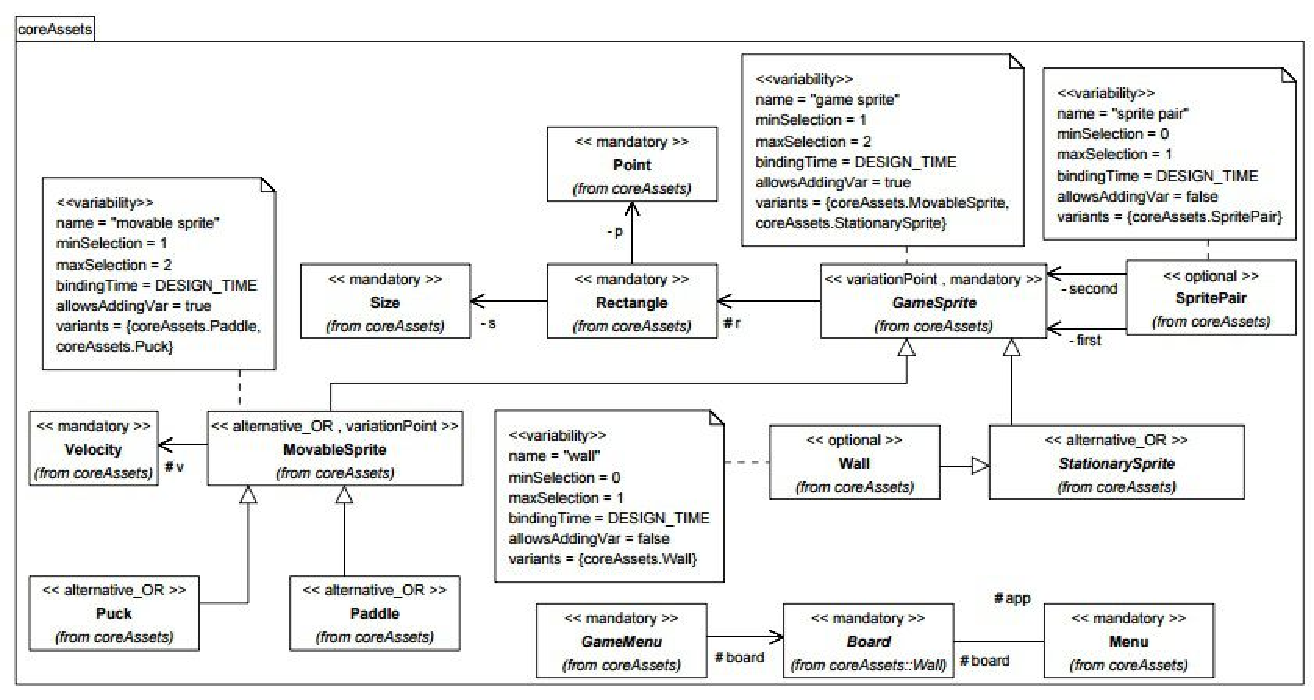
\includegraphics[height=10cm, width=16cm]{AGM_Class_Variability_Model.pdf}
\end{figure}

A relação entre variabilidades, pontos de variação e variantes pode ser percebida claramente na \ref{AGM}. Considerando a classe \textit{GameSprite} presente na figura, percebe-se os estereótipos $<<\textit{variationPoint}>>$ e $<<\textit{mandatory}>>$, indicando que a classe é um ponto de variação e simultaneamente uma variante obrigatória. Por ser um ponto de variação, tal classe está associada com uma variabilidade, no caso o comentário \textit{game sprite}, estereotipado com $<<\textit{variability}>>$. Duas variantes estão associadas ao ponto de variação, \textit{StationarySprite} e \textit{MovableSprite}, ambas estereotipadas com $<<\textit{alternative\_OR}>>$. Outros estereótipos também são observados, tais como o $<<\textit{optional}>>$, na classe \textit{SpritePair} e o $<<\textit{alternative\_OR}>>$, nas classes \textit{Puck} e \textit{Paddle}. Na geração de um produto por exemplo, o arquiteto de LPS pode escolher se o produto conterá elementos estáticos (\textit{StationarySprite}), móveis (\textit{MovableSprite}) ou mesmo ambos no jogo gerado.